\documentclass[12pt]{article}

\usepackage{tikz} % картинки в tikz
\usepackage{microtype} % свешивание пунктуации
\usepackage{array} % для столбцов фиксированной ширины
\usepackage{comment} % для комментирования целых окружений
\usepackage{indentfirst} % отступ в первом параграфе

\usepackage{sectsty} % для центрирования названий частей
\allsectionsfont{\centering}

\usepackage{amsmath, amssymb, amsthm, amsfonts} % куча стандартных математических плюшек

\usepackage[top=2cm, left=1cm, right=1cm, bottom=2cm]{geometry} % размер текста на странице
\usepackage{lastpage} % чтобы узнать номер последней страницы
 
\usepackage{enumitem} % дополнительные плюшки для списков
%  например \begin{enumerate}[resume] позволяет продолжить нумерацию в новом списке

\usepackage{caption} % подписи к рисункам
\usepackage{hyperref} % гиперссылки
\usepackage{multicol} % текст в несколько столбцов


\usepackage{fancyhdr} % весёлые колонтитулы
\pagestyle{fancy}
\lhead{Введение в машинное обучение, ВШЭ}
\chead{}
\rhead{2022-04-25}
\lfoot{Вариант $\Sigma \Theta \Kappa$}
\rfoot{Паниковать запрещается!}
%\rfoot{Тест}
\renewcommand{\headrulewidth}{0.4pt}
\renewcommand{\footrulewidth}{0.4pt}

\usepackage{ifthen} % для написания условий

\usepackage{todonotes} % для вставки в документ заметок о том, что осталось сделать
% \todo{Здесь надо коэффициенты исправить}
% \missingfigure{Здесь будет Последний день Помпеи}
% \listoftodos --- печатает все поставленные \todo'шки


% более красивые таблицы
\usepackage{booktabs}
% заповеди из докупентации:
% 1. Не используйте вертикальные линни
% 2. Не используйте двойные линии
% 3. Единицы измерения - в шапку таблицы
% 4. Не сокращайте .1 вместо 0.1
% 5. Повторяющееся значение повторяйте, а не говорите "то же"


\usepackage{fontspec}
\usepackage{polyglossia}

\setmainlanguage{russian}
\setotherlanguages{english}

% download "Linux Libertine" fonts:
% http://www.linuxlibertine.org/index.php?id=91&L=1
\setmainfont{Linux Libertine O} % or Helvetica, Arial, Cambria
% why do we need \newfontfamily:
% http://tex.stackexchange.com/questions/91507/
\newfontfamily{\cyrillicfonttt}{Linux Libertine O}

% Математические шрифты 
% Математические шрифты 
\usepackage{unicode-math}     
\setmathfont[math-style=upright]{euler.otf} 

\setmathfont[range={\mathbb, \mathop, \heartsuit, \angle, \smile, \varheartsuit}]{Asana-Math.otf}

\AddEnumerateCounter{\asbuk}{\russian@alph}{щ} % для списков с русскими буквами
\setlist[enumerate, 2]{label=\asbuk*),ref=\asbuk*}


% мои цвета https://www.artlebedev.ru/colors/
\definecolor{titleblue}{rgb}{0.2,0.4,0.6} 
\definecolor{blue}{rgb}{0.2,0.4,0.6} 
\definecolor{red}{rgb}{1,0,0.2} 
\definecolor{green}{rgb}{0,0.6,0} 
\definecolor{purp}{rgb}{0.4,0,0.8} 

% цвета из geogebra 
\definecolor{litebrown}{rgb}{0.6,0.2,0}
\definecolor{darkbrown}{rgb}{0.75,0.75,0.75}

% Гиперссылки
\usepackage{xcolor}   % разные цвета

\usepackage{hyperref}
\hypersetup{
  unicode=true,           % позволяет использовать юникодные символы
  colorlinks=true,        % true - цветные ссылки
  urlcolor=blue,          % цвет ссылки на url
  linkcolor=black,          % внутренние ссылки
  citecolor=green,        % на библиографию
  breaklinks              % если ссылка не умещается в одну строку, разбивать её на две части?
}

% эпиграфы
\usepackage{epigraph}
\setlength\epigraphwidth{.7\textwidth}
\setlength\epigraphrule{0pt}

% Математические операторы первой необходимости:
\DeclareMathOperator{\sgn}{sign}
\DeclareMathOperator*{\argmin}{arg\,min}
\DeclareMathOperator*{\argmax}{arg\,max}
\DeclareMathOperator{\Cov}{Cov}
\DeclareMathOperator{\Var}{Var}
\DeclareMathOperator{\Corr}{Corr}
\DeclareMathOperator{\E}{\mathop{E}}
\DeclareMathOperator{\Med}{Med}
\DeclareMathOperator{\Mod}{Mod}
\DeclareMathOperator*{\plim}{plim}

\DeclareMathOperator{\logloss}{logloss}
\DeclareMathOperator{\softmax}{softmax}

\DeclareMathOperator{\tr}{tr}

% команды пореже
\newcommand{\const}{\mathrm{const}}  % const прямым начертанием
\newcommand{\iid}{\sim i.\,i.\,d.}  % ну вы поняли...
\newcommand{\fr}[2]{\ensuremath{^{#1}/_{#2}}}   % особая дробь
\newcommand{\ind}[1]{\mathbbm{1}_{\{#1\}}} % Индикатор события
\newcommand{\dx}[1]{\,\mathrm{d}#1} % для интеграла: маленький отступ и прямая d

% одеваем шапки на частые штуки
\def \hb{\hat{\beta}}
\def \hs{\hat{s}}
\def \hy{\hat{y}}
\def \hY{\hat{Y}}
\def \he{\hat{\varepsilon}}
\def \hVar{\widehat{\Var}}
\def \hCorr{\widehat{\Corr}}
\def \hCov{\widehat{\Cov}}

% Греческие буквы
\def \a{\alpha}
\def \b{\beta}
\def \t{\tau}
\def \dt{\delta}
\def \e{\varepsilon}
\def \ga{\gamma}
\def \kp{\varkappa}
\def \la{\lambda}
\def \sg{\sigma}
\def \tt{\theta}
\def \Dt{\Delta}
\def \La{\Lambda}
\def \Sg{\Sigma}
\def \Tt{\Theta}
\def \Om{\Omega}
\def \om{\omega}

% Готика
\def \mA{\mathcal{A}}
\def \mB{\mathcal{B}}
\def \mC{\mathcal{C}}
\def \mE{\mathcal{E}}
\def \mF{\mathcal{F}}
\def \mH{\mathcal{H}}
\def \mL{\mathcal{L}}
\def \mN{\mathcal{N}}
\def \mU{\mathcal{U}}
\def \mV{\mathcal{V}}
\def \mW{\mathcal{W}}

% Жирные буквы
\def \mbb{\mathbb}
\def \RR{\mbb R}
\def \NN{\mbb N}
\def \ZZ{\mbb Z}
\def \PP{\mbb{P}}
\def \QQ{\mbb Q}

\def \putyourname{\fbox{
    \begin{minipage}{42em}
      Фамилия, имя, номер группы:\vspace*{3ex}\par
      \noindent\dotfill\vspace{2mm}
    \end{minipage}
  }
}

\def \checktable{

  \vspace{5pt}
  Табличка для проверяющих работу:

\vspace{5pt}

  \begin{tabular}{|m{2cm}|m{1cm}|m{1cm}|m{1cm}|m{1cm}|m{1cm}|m{1cm}|m{1cm}|m{2cm}|}
\toprule
    Задачи & 1 & 2 & 3 & 4 & 5 & 6 & 7 & Итого \\
\midrule
    &  &  & & & & & & \\
    &  &  & & & & & & \\
 \bottomrule
\end{tabular}
}


\def \testtable{

\vspace{5pt}
  Внесите сюда ответы на тест:

\vspace{5pt}

\begin{tabular}{|m{2cm}|m{0.6cm}|m{0.6cm}|m{0.6cm}|m{0.6cm}|m{0.6cm}|m{0.6cm}|m{0.6cm}|m{0.6cm}|m{0.6cm}|m{0.6cm}|}
\toprule
    Вопрос & 1 &  2 & 3 & 4 & 5 & 6 & 7 & 8 & 9 & 10 \\
\midrule
    Ответ &  &  & & & & & & & & \\
 \bottomrule
\end{tabular}
}


% [1][3] 1 = one argument, 3 = value if missing
% эта магия создаёт окружение answerlist
% именно в окружении answerlist записаны варианты ответов в подключаемых exerciseXX
% просто \begin{answerlist} сделает ответы в три столбца
% если ответы длинные, то надо в них руками сделать
% \begin{answerlist}[1] чтобы они шли в один столбец
\newenvironment{answerlist}[1][3]{
\begin{multicols}{#1}

\begin{enumerate}[label=\fbox{\emph{\Alph*}},ref=\emph{\alph*}]
}
{
\item Нет верного ответа.
\end{enumerate}
\end{multicols}
}

% BB: unicol version. don't know why \ifthenelse fails in second part of new-env
\newenvironment{answerlistu}{
\begin{enumerate}[label=\fbox{\emph{\Alph*}},ref=\emph{\alph*}]
}
{
\item Нет верного ответа.
\end{enumerate}
}


\excludecomment{solution} % without solutions

\theoremstyle{definition}
\newtheorem{question}{Вопрос}

\usepackage{tikzlings}
\usepackage{tikzducks}

\usepackage{alltt}

\begin{document}

\putyourname

\testtable

\checktable

\epigraph{Позитивная мотивация — явно не мой конёк, и мы все умрём. \\ Всё уже было до нас, можно выдохнуть страх, и уставить глаза в небосклон. \\ Если этой контрольной и сопротивляться, то не с печальным лицом. \\ Всё повторится не раз, но мы живы сейчас, нами рано удобрять чернозём.}{\textit{Oxxxymiron и Тося Чайкина про мидтёрм по ML (2022)}}


Работа состоит из трёх частей: тестовая, задачи и ответы на открытые вопросы. Списывание карается обнулением работы. Удачи!


\section*{Часть первая: тестовая} 

Дайте ответ на $10$ тестовых вопросов. Каждый вопрос стоит $3$ балла. Никакие дополнительные пояснений в этой части работы от вас не требуются.

\begin{question}
Архимед хочет отбить римскую атаку на Сиракузы. С помощью беспилотника Архимед делает съёмки римских кораблей, а затем специальным алгоритмом компьютерного зрения пытается предсказать, сколько римских солдат находится на каком корабле. Какую задачу решает Архимед? 
\begin{answerlist}
   \item  Регрессия
   \item  Классификация
   \item  Кластеризация
   \item  Ранжирование
   \item  Рекомендаии
\end{answerlist}
\end{question}

\begin{solution}
\begin{answerlist}
  \item Good answer :)
  \item Bad answer :(
  \item Bad answer :(
  \item Bad answer :(
  \item Bad answer :(
\end{answerlist}
\end{solution}


\begin{question}
Что такое гиперпараметр?
\begin{answerlist}
  \item Параметр, который оказывает ключевое влияние на производительность модели
  \item Ровно то же самое, что и параметр
  \item Параметр, чьё оптимальное значение нельзя подобрать по обучающей выборке
  \item Параметр, который является многомерным
  \item Параметр, от которого выход модели зависит нелинейно
\end{answerlist}
\end{question}

\begin{solution}
\begin{answerlist}
  \item Bad answer :(
  \item Bad answer :(
  \item Good answer :)
  \item Bad answer :(
  \item Bad answer :(
\end{answerlist}
\end{solution}

\newpage 

\begin{question}
В чём потенциальный недостаток кросс-валидации по двум блокам?

\begin{answerlist}
   \item Оценка качества модели на новых данных может оказаться очень заниженной из-за того, что тестирование проводится на слишком маленькой выборке
   \item Оценка качества модели на новых данных может оказаться очень заниженной из-за того, что тестирование проводится на слишком большой выборке
   \item Оценка качества модели на новых данных может оказаться очень заниженной из-за того, что обучение проводится на выборке сильно больше исходной
  \item Оценка качества модели на новых данных может оказаться очень заниженной из-за того, что обучение проводится на выборке сильно меньше исходной
  \item Нужно обучать слишком много моделей, вычислительных мощностей для этого может не хватить, новые сервера в Россию из-за санкций не поставляют, поэтому кросс-валидация по двум блокам не имеет никакого смысла
\end{answerlist}
\end{question}

\begin{solution}
\begin{answerlist}
  \item Good answer :)
  \item Bad answer :(
  \item Bad answer :(
  \item Good answer :)
  \item Good answer :)
\end{answerlist}
\end{solution}



\begin{question}
Что из этого формула для шага в градиентном спуске? 
\begin{answerlist}
  \item \(w_t = w_{t-1} - \eta \cdot \nabla L(w_{t})\) 
  \item \(w_t = w_{t-1} + \eta \cdot \nabla L(w_{t})\)
  \item \(w_t = w_{t-1} - \eta \cdot \nabla L(w_{t-1})\)
  \item \(w_t = w_{t-1} - \eta \cdot \nabla L(w_{0})\)
  \item \(w_t = w_{t-1} + \eta \cdot \nabla L(w_{t-1})\) 
\end{answerlist}
\end{question}
\begin{solution}
\begin{answerlist}
  \item Bad answer :(
  \item Bad answer :(
  \item Good answer :)
  \item Bad answer :(
  \item Bad answer :(
\end{answerlist}
\end{solution}


\begin{question}
Какие из сопособов приведённых ниже можно использовать для работы с пропусками в категориальных переменных при обучении линейных моделей? 
\begin{answerlist}
   \item Если пропусков очень много, выкинуть переменную 
   \item Заполнить пропуски аномальным значением
   \item Выделить пропуски в отдельную категорию и сделать OHE-преобразование
  \item Заполнить нулями 
  \item Заполнить пропуски медианами, посчитанными по каждой колонке 
\end{answerlist}
\end{question}

\begin{solution}
\begin{answerlist}
  \item Good answer :)
  \item Bad answer :(
  \item Good answer :)
  \item Bad answer :(
  \item Bad answer :(
\end{answerlist}
\end{solution}


\begin{question}
Бог плодородия Дионис спустился с Олимпа вкусить вина свежего урожая. Зевс пытается понять, сколько дней будет идти кутёж Диониса. Для этого он использует линейную регрессию, обученную на предыдущих кутежах:

\[ 
y_i = 7 + 0.5 \cdot x_1 + 0.2 \cdot x_2,
\]

где $x_1$ --- качество вина по десятибальной шкале, $x_2$ --- количество событульников. Выберите все верные утверждения об этой модели.

\begin{answerlist}
   \item  Каждые дополнительные $5$ собутыльников будут затягивать кутёж на день
   \item  In vino veritas, in aqua sanitas
   \item  Кутёж затянется минимум на $14$ дней
   \item  Кутёж затянется минимум на $7$ дней
   \item  Каждый дополнительный собутыльник будет затягивать кутёж на один день 
\end{answerlist}
\end{question}

\begin{solution}
\begin{answerlist}
  \item Good answer :)
  \item Good answer :)  
  \item Bad answer :(
  \item Good answer :)
  \item Bad answer :(
\end{answerlist}
\end{solution}

\newpage 

\begin{question}
Что из этого можно использовать для регуляризации?
Под регуляризацией мы понимаем штрафование моделей за сильно отличающиеся от нуля веса.
\begin{answerlist}
   \item  \( |w_1| + |w_2| + \ldots + |w_d| \)
   \item  \( \frac{1}{|w_1|} + \frac{1}{|w_2|} + \ldots + \frac{1}{|w_d|} \)
   \item  \( w_1^2 + w_2^2 + \ldots + w_d^2 \)
   \item  \( w_1^3 + w_2^3 + \ldots + w_d^3 \)
   \item  \( |w_1|^3 + |w_2|^3 + \ldots + |w_d|^3 \)
\end{answerlist}
\end{question}

\begin{solution}
\begin{answerlist}
  \item Good answer :)
  \item Bad answer :(
  \item Bad answer :(
  \item Good answer :)
  \item Good answer :)
\end{answerlist}
\end{solution}


\begin{question}
У нас есть $2$ класса. Классификатор предсказывает, что объект равновероятно относится к каждому из них. Какое значение принимает logloss на этом объекте? 
\begin{answerlist}
  \item \(-\log 2 \)
  \item \(-0.5 \log 2 \)
  \item \(-2 \log 2 \)
  \item \(-2 \log 0.5 \)
  \item \(\log 2\)
\end{answerlist}
\end{question}

\begin{solution}
\begin{answerlist}
  \item Bad answer :(
  \item Bad answer :(
  \item Bad answer :(
  \item Bad answer :(
  \item Good answer :)
\end{answerlist}
\end{solution}


\begin{question}
Леонид предсказывает цены на квартиры в Спарте с помощью метода ближайших соседей. При построении предсказания он хочет учитывать расстояние до соседей. Какая из формул ниже поможет Леониду корректно построить прогноз?  Все суммы ищутся по ближайшим соседям, $y_j$ --- цена квартиры, $\rho_j$ --- расстояние от объекта для которого строится предсказание до соотвествующего соседа.
\begin{answerlist}
   \item \(\frac{1}{k} \sum_{j=1}^k y_j\)
   \item \(\frac{\sum_{j=1}^k \rho_j \cdot y_j }{\sum_{j=1}^k \rho_j} \) 
   \item \(\frac{1}{k} \sum_{j=1}^k \frac{y_j}{\rho_j} \) 
   \item \(\frac{\sum_{j=1}^k \rho_j \cdot y_j }{\sum_{j=1}^k \tfrac{1}{\rho_j}} \) 
   \item \(\frac{\sum_{j=1}^k \tfrac{1}{\rho_j} \cdot y_j }{\sum_{j=1}^k \rho_j} \)
\end{answerlist}
\end{question}

\begin{solution}
\begin{answerlist}
  \item Bad answer :(
  \item Bad answer :(
  \item Bad answer :(
  \item Bad answer :(
  \item Bad answer :(
\end{answerlist}
\end{solution}


\begin{question}
Какие из метрик перечисленных ниже используются для решения задачи классификации? 
\begin{answerlist}
   \item  MSE
   \item  f-мера
   \item  MAPE
   \item  logloss
   \item  ROC-AUC 
\end{answerlist}
\end{question}

\begin{solution}
\begin{answerlist}
  \item Bad answer :(
  \item Good answer :)
  \item Bad answer :(
  \item Good answer :)
  \item Good answer :)
\end{answerlist}
\end{solution}




\newpage 

 
\section*{Часть вторая: открытые вопросы}

Эта часть состоит из открытых вопросов. На них необходимо дать краткие, но ёмкие ответы. За каждый ответ вы можете получить 10 баллов.

\begin{question}
Предложите для каждой из перечисленных ниже задач, как сформулировать их в терминах машинного обучения: укажите, что будет являться объектом и целевой переменной, а также напишите тип задачи.

\begin{enumerate}
    \item В заповеднике голод --- белки часто остаются некормленными, так как зайцы оказываются слишком прожорливыми и съедают чужую еду. Мы приняли решение поставить кормушки с фотоловушками, которые бы открывались для того животного, которое подошло к кормушке, чтобы ограничить ненасытных зайцев.
  \item По статистике некоторая доля сотрудников одной компании ежедневно опаздывает из-за пробок, сокращая свой рабочий день на некоторое количество времени. Мы решили разработать приложение, которое будет подсказывать сотрудникам, на какое время им стоит запланировать выход из дома, чтобы не опоздать на работу.
\end{enumerate}
\end{question}


\vspace{4cm} 



\begin{question}
Аполоний обожает логистическую регрессию. Поэтому он решил закодить её самостоятельно, без всяких пакетов. Он записал модель следующим образом: 

\begin{equation*} 
\begin{aligned}
    & b(x_i) = \sigma(b + \langle x_i, w \rangle) \\
    & \sigma(t) = \frac{1}{1 - exp(t)}
\end{aligned}
\end{equation*}

Для обучения Аполоний использует функцию потерь 

\[
L(b(x_i), y_i) = b(x_i \cdot \ln y_i + (1 - b(x_i) \cdot \ln (1 - y_i)
\]

Какие ошибки вы тут видите? Для каждой объясните, к каким последствиям и почему она приведёт, а также как это исправить.
\end{question}


\newpage 

\begin{question}
Объясните мем
\begin{center}
  
\includegraphics[scale=0.9]{memes2.jpg}
\end{center}
\end{question}


\vspace{6cm} 


\begin{question}
Пигмалион оживил Галатею, вырезанную из слоновой кости! Теперь они хотят обучить метод ближайших соседей для классификации горных пород. В качестве признаков используются: вес пород, размер, цвет и тп. 

Галатея хочет строить свои прогнозы с учётом того, каким получилось расстояние между объектами. Пигмалион хочет строить свои прогнозы с помощью метода большинства. Выпишите формулы, которые будут использованы для расчёта прогнозов. Объясните в них каждую компоненту и обозначения. 
\end{question}

\vspace{5cm} 

\newpage 

\begin{question}
Аргонавты плавают вокруг нимф и пытаются понять, сколько их нужно слушать, чтобы весь экипаж зачаровало. По собранным данным оценивается линейная регрессия. В качестве объясняющей переменной, $x$ используется длина песни, в качестве объясняемой число зачарованных аргонавтов, $y$.  В качестве функции потерь используется $MSE.$ 

Ясон отложил по оси $x$ длину песни, а по оси $y$ число зачарованных аргонавтов. Поверх облака точек он нарисовал линейную регрессию. Получилась такая картинка: 
\begin{center}
  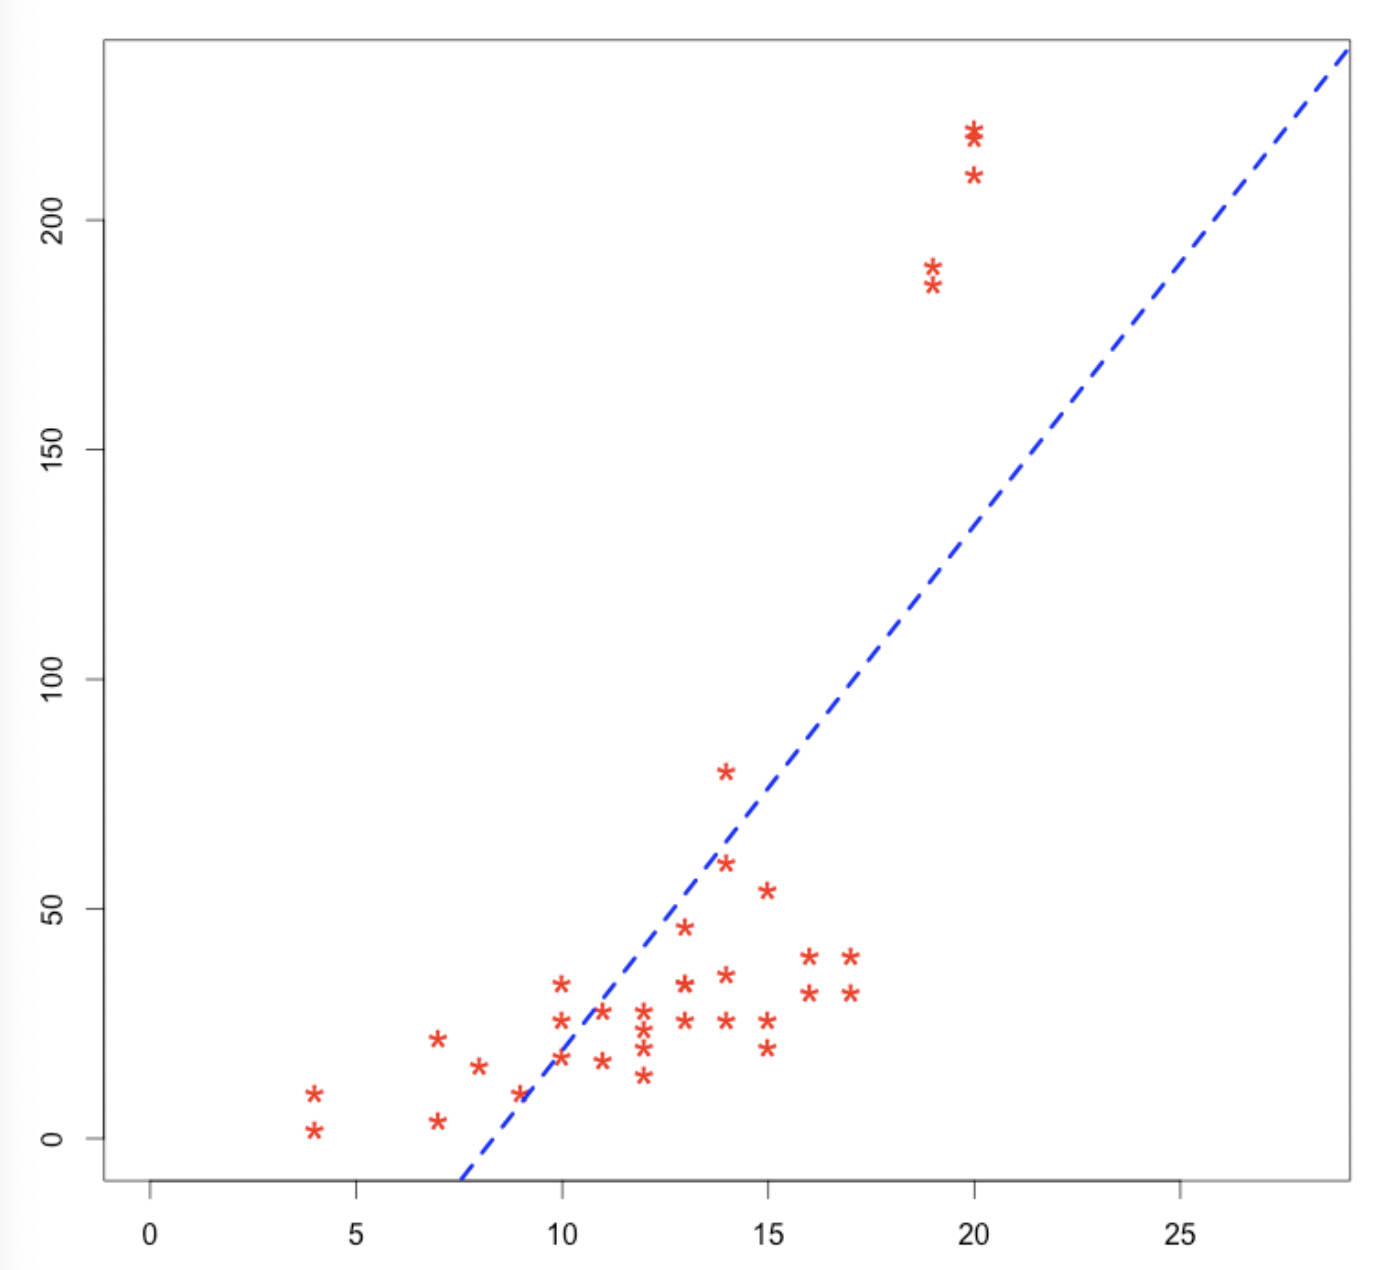
\includegraphics[scale=0.4]{out.png}
\end{center}
\end{question}

С какими проблемами при обучении модели столкнулся Ясон? Предложите как минимум два способа исправить возникшую проблему. 

\vspace{5cm} 



\newpage 

\section*{Часть третья: задачки}

Решите все задания. Все ответы должны быть обоснованы. Решения должны быть прописаны для каждого пункта. Рисунки должны быть чёткими и понятными. Все линии должны быть подписаны. За решение каждой задачи вы можете получить 10 баллов.

\begin{question}
Мойры предсказывают судьбу. Клото использует для этого метод ближайших соседей. Ла́хеси использует линейную регрессию, а А́тропо случайный лес. В тестовой выборке у них есть три наблюдения $y_i$. Для каждого из них мойры построили прогнозы. 

\begin{center}
  \begin{tabular}{c|c|c|c}
    настоящие $y_i$ &  1 & 2 & 3 \\
    \hline
    KNN & 2 & 3 & 1  \\
    линейная регрессия &  2 & 3 & 4 \\
    случайный лес & 1 & 1 & 1 \\
  \end{tabular}
\end{center}

\begin{enumerate}
    \item Найдите для прогнозов $MAE$, $MSE$, $RMSE$ и $MAPE$.
    \item Объясните, зачем от $MSE$ обычно переходят к $RMSE$.
    \item Объясните, почему $MAE$ считается более устойчивой к выбросам.
\end{enumerate}
\end{question}

\newpage 

\begin{question}
    Константин основал Константинополь, а затем решил задачу классификации. У него получились следующие прогнозы. 
    
    \begin{center}
      \begin{tabular}{c|c}
        $y_i$ & $\hat p_i$ \\
        \hline
        $1$  & $0.9$ \\
        $1$ & $0.1$ \\
        $0$ & $0.75$ \\
        $1$ & $0.56$ \\
        $0$ & $0.2$ \\
        $0$ & $0.37$ \\
        $0$ & $0.25$ \\   
      \end{tabular}
    \end{center}
    
    \begin{enumerate}
      \item  Бинаризуйте ответ по порогу $t$ и посчитайте точность и полноту для $t = 0.3$ и для  $t = 0.8$.
      \item Постройте ROC-кривую и найдите площадь под ней. 
    \end{enumerate}
\end{question}


\end{document}




